\section{Introduction }
%Dans le cadre du module Initiation à la recherche, 
L'objectif de ce document est de décrire les notions essentielles à retenir en ce début de projet d'initiation à la recherche. Ces notions font partie d'un même sujet d'étude, au cœur des travaux de l'équipe OPTI. Elles concernent le sujet des contraintes et des intervalles. %Aussi des notions d'optimisation seront abordées.

\section{Présentation du problème}
\subsection{Définition du contexte}
Un problème de satisfaction de contraintes (CSP) est défini par 3 éléments : 
\begin{itemize}
\item
Un ensemble de variables $\mathbf{V} = \left\{ v_1,...,v_n \right\}$.
\item
Un domaine de valeurs pour chaque variable. Chaque valeur du domaine $D_i$ associé à la variable $v_i$ est une valeur que peut potentiellement prendre $v_i$ : $\mathbf{D} = D_1 \times ... \times D_n $.
\item
Un ensemble de contraintes (relations) $\mathbf{C}$ restreignant les variables de $\mathbf{V}$ défini ci-dessus :  $\mathbf{C} = \left\{c_1,...,cm\right\}$. 
\end{itemize}

On s'intéressera notamment à la résolution des CSP sur le domaine continu. Dans ce cas les variables seront des intervalles à valeurs réelles et les contraintes seront généralement représentées par des équations et des inégalités. 


\subsection{Exemple}

Une représentation simple de ce type de problèmes est la recherche des intersections de deux cercles dans un plan : 
\begin{figure}[h] %on ouvre l'environnement figure
  \center
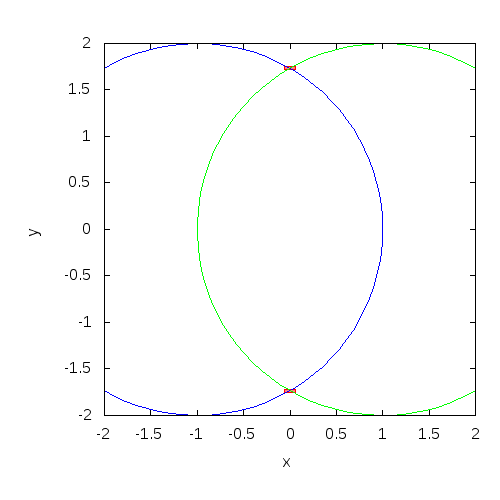
\includegraphics[scale=0.43]{img/circle-circle}
  \caption{Intersection de deux cercles} %la légende
 \label{fig:Deuxcerlces} %la légende
\end{figure} %on ferme l'environnement figure

Définissons deux cercles respectivement de rayons  $r_1$ et $r_2$ et de centres : $(x_1,y_1)$ et $(x_2,y_2)$.
On peut alors fixer les données en entrées du problème :

\begin{itemize}
\item
Un ensemble de variables $\{x,y\}$ .
\item
Un domaine de valeurs pour chaque variable. 
\item
Les constantes du problème : les rayons de chaque cercle situés dans  $\mathbb{R⁺}$.
\item
L'ensemble des contrainte est composé par les équations des cercles :
\begin{equation}\label{eq}
\begin{cases}
(x-x_1)²+(y-y_1)² = r_1²\\
(x-x_2)²+(y-y_2)² = r_2²
\end{cases}
\end{equation}




\end{itemize}
%\clearpage


\section{Méthodes de calculs}
Les méthodes de calculs permettent la résolution de problèmes mathématiques en machine; en particulier lorsque l'on cherche à résoudre des problèmes sur les nombres réels. Elles permettent par exemple la résolution des CSP  ou GCSP (Geometric Constraint Satisfaction Problem \cite{Jermann}) et peuvent être divisées en deux catégories : les méthodes formelles et les méthodes numériques. . 


\subsection{Méthodes formelles}
Les méthodes formelles permettent de résoudre des système d'équations ou d'inéquations en utilisant au maximum le calcul symbolique. Les approches les plus classiques des méthodes formelles utilisent des théories, telles que les idéaux polynomiaux pour les bases de Gröbner, ou la théorie des déterminants pour la méthode du résultant.

 Ces méthodes ont l'énorme avantage de retourner des solutions exactes d'un système d'équation, ou tout du moins de minimiser l'utilisation de l'arithmétique flottante. Elles tenteront donc de résoudre le problème (\ref{eq}) en effectuant uniquement des opérations sur les équations sans évaluer les variables. On pourra donc avoir des expressions pour $x$ et $y$ représentant les solutions du problème de façon symbolique. 

Cependant les résolutions de problèmes par des méthodes formelles sont forcément restreintes par les possibilités du calcul symbolique et ne pourront donc pas toujours offrir de solution générale \textbf{et de mettre en œuvre des algorithmes de complexité exponentielles.} Il n'existe par exemple pas de formule générale permettant de trouver les solutions d'un polynôme de degré supérieur ou égal à cinq.


\subsection{Méthodes numériques}
Les méthodes numériques consistent à évaluer de façon calculatoire la ou les solutions d'un problème. En effet elles sont capables d'essayer de résoudre n'importe quel système d'équation (ou d'égalités). Ainsi dans le cas du problème (\ref{eq}) la machine va affecter directement les calculs pour évaluer le résultats. Or l'utilisation de la représentation flottante et de son arithmétique pour simuler les opérations réelles va entrainer une diffusion et une augmentation de l'erreur de calcul, à tel point que l'on ne peut  parfois plus assurer la validité d'une solution. On pourra d'ailleurs citer à titre d'exemple le problème de l'inversion d'une matrice mal conditionnée\cite{Conditionnement}. 

Cependant ces calculs numériques utilisés  par des méthodes de résolutions par intervalles permettent de contourner ces problèmes. Pour plus de détails sur la représentation flottante, on pourra se référer à la thèse de Frédéric Goualard \cite{Goualard}

